\documentclass{article}
\usepackage{bigstrut}
\usepackage{adjustbox}
\usepackage{graphicx}^^M
\graphicspath{ {images/} }
\usepackage[T1]{fontenc}
\usepackage{float}

\usepackage[english]{babel}
\usepackage[utf8]{inputenc}
\usepackage{indentfirst}

\addtolength{\oddsidemargin}{-.875in}
\addtolength{\evensidemargin}{-.875in}
\addtolength{\textwidth}{1.75in}
\addtolength{\textheight}{1in}

\begin{document}
\title{Design V: Lab 4}
\begin{titlepage}
    \centering
	{\scshape\LARGE Lab 4: Thermo-Mechanical Processing of Aluminum\par}
	\vspace{1cm}
	{\scshape Aristide Muscariello Jr.: Technician,Recorder \hfill ID\#:10406472 \par}
	{\scshape Marcin Wisniowski: Manager,Technician \hfill ID\#:10417225\par}
	\vfill
	{\scshape Design V, Week 4\par}
	\vspace{.5cm}
	{\scshape Laboratory Performed: February 13th, 2018\\Stevens Institute of Technology\\E-231 Section I Group 3\par}
	\vspace{.5cm}
	{\scshape supervised by\\Mr. Di Wu, Mr. Kai Zong \par}
    \vfill
% Bottom of the page
	{\scshape“I pledge my honor that I have abided by the Stevens Honor System.”\par}
	\vspace{.5cm}
	{\scshape Aristide Muscariello Jr. \hfill Date: 02/19/18\\Marcin Wisniowski \hfill Date: 02/19/18\\}
	\vspace{3cm}
\end{titlepage}

\section{Introduction}
For this experiment, there were several goals to be achieved.  The group would first describe the basic principles of an automatic indentation instrument, while using the machine to perform hardness tests. Using the results from this, the team would describe the change in the mechanical properties of aluminum due to both cold rolling and thermal annealing. The final goal of the lab was to use an optical microscope to observe and describe metallography changes in aluminum due to cold rolling.

\subsection{Objectives}
\begin{enumerate}
\item Describe the  basic principles of and be able to perform hardness test using automated indentation instrument
\item Be able to describe the change in mechanical properties due to both cold rolling and thermal annealing
\item Use an optical microscope to observe and qualitatively describe changes in metallographic due to cold rolling
\item Select a metal or alloy for a particular structural application based on mechanical properties which can be modified by thermo-mechanical processing
\end{enumerate}

\subsection{Hypothesis}
The group believes that after annealing a metal will increase its hardness. On the other hand, the group believes that lowering the thickness will cause the material to lower in the hardness scale. 

\section{Procedure}
\subsection {Hardness Tests on Aluminum Alloys}
\indent The first part of the lab involved the use of an automated indentation instrument which would aid the team in performing a Rockwell H hardness test. The machine would indent a piece of either aluminum 3003 or 6061 5 times, recording the hardness each time. The repetition of this beginning experiment will allow a more accurate data point of the hardness of aluminum by allowing the team to take an average of the results found. After performing the experiment on the 2 know pieces, a 3rd unknown piece of aluminum would be tested in the machine.

\subsection{Thermal Annealing in Unknown Aluminum Alloy}
\indent Continuing off of the first experiment, the second experiment to be run by the group will continue testing on the unknown piece of aluminum. After being indented 5 times during the hardness test, the unknown piece of aluminum was placed in an annealing furnace set to 400$^o$C for 1 hour. After the time had passed, the aluminum was recovered and set aside to cool before being placed in the machine to once again test its hardness. 5 additional measurements were made. Meanwhile, one of the 2 know pieces of aluminum was to undergo cold rolling. The sample’s initial thickness was measured before being sent through the machine, which would theoretically reduce the sample’s thickness by 10\% each time it was sent through. After being sent through, the sample was placed back into the hardness tester and another 5 indents/readings were taken. This whole process, cold rolling followed by hardness testing, was repeated until the sample would no longer be able to pass through the machine without breaking. Measurements were taken following each pass through the cold rolling machine.
	
\subsection{Observation of Microstructure Changes during Cold Rolling}
\indent Finally, the third experiment would have the lab group observe two prepared metallography specimens under a microscope. One sample will be as-cast while the other will be of identical composition, but have been cold rolled enough times to reduce the overall thickness to 50\%. The supplied microscope will be used to capture a digital image of both samples at 5x and 20x magnification. The MotiConnection image software allows the lab team to drag a scale bar with a known length on the captured image, which will be used for further analysis of the images.

\section{Results}

\subsection{Cold Working}
The group initially received a sample of a 3003 Aluminum Alloy Sample, and this was placed through a roller. Below, the table shows how cold-rolling the metal increased the hardness of the material. As the thickness lowered, the average hardness increased, while the standard deviation stayed relatively similar.

\begin{center}
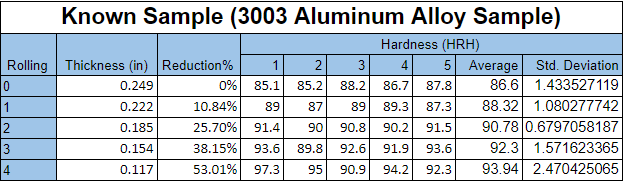
\includegraphics[width=450pt]{Lab4Data.png}
\end{center}

\begin{center}
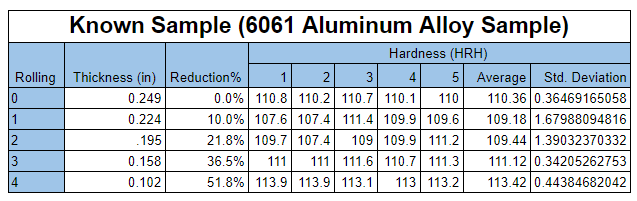
\includegraphics[width=450pt]{Lab4Data2.png}
\end{center}

Both specimens appear to have similar growths in hardness after cold-working, but after further analysis, the 3003 sample gains its hardness twice as fast as the 6061 sample. The trend lines show that sample 3003 has a gain of approximately 1.4165 hardness every 10\% cold-working rolling, while sample 6061 gains .66285 per 10\% cold-working rolling. However, while the 6061 Aluminum sample increases slower in hardness, it also starts at a higher hardness by over 20 on the Rockwell H hardness scale. 

\begin{center}
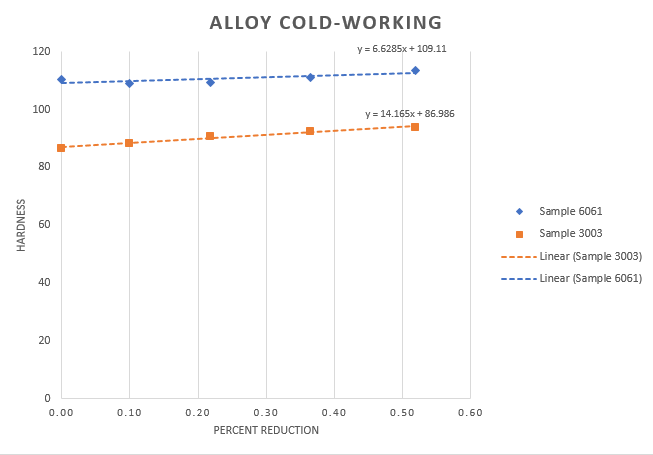
\includegraphics[width=450pt]{AlloyColdWorking.png}
\end{center}


\subsection{Annealing}

\indent The annealing process increases the hardness of a material.Before the annealing process of our unknown material, the average hardness was 112.2 on the Rockwell scale, but after annealing it lowered to 57.34. This is because the annealing process allows a material to return back to its initial properties before cold-working affect them and recreating their structural properties. This material was most likely a sample of 6061 aluminum which had been cold-worked to approximately 40\% reduction, because the value of 112.2 is closest to the 36.5\% reduction of Sample 6061 (111.12). Ultimately, however, the inconsistent data does not allow the group to decide what material it was before annealing.

\indent There may have been errors when finding this data, but because our group was only given the dataset, nothing could have been fixed. It is important to note that the standard deviation of the annealed metal was much larger than before annealing, showing that the material was not completely similar in hardness across the whole surface. Similarly, the known samples have been reused by multiple lab groups and should have also been annealed along with the unknown sample to reset their hardness to initial conditions. The unknown sample could have been either sample 6061 or Sample 3003. The values of the sample were very similar to Sample 6061 before annealing, but after annealing they appeared closer to Sample 3003. 

\begin{center}
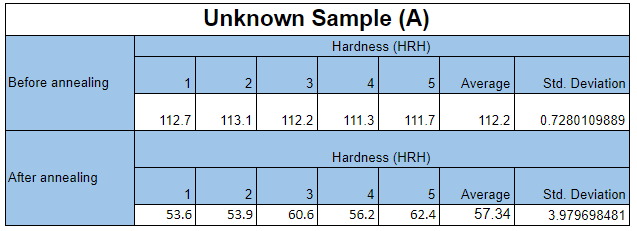
\includegraphics[width=400pt]{Annealing.png}
\end{center}

\subsection{Observations}

\begin{center}
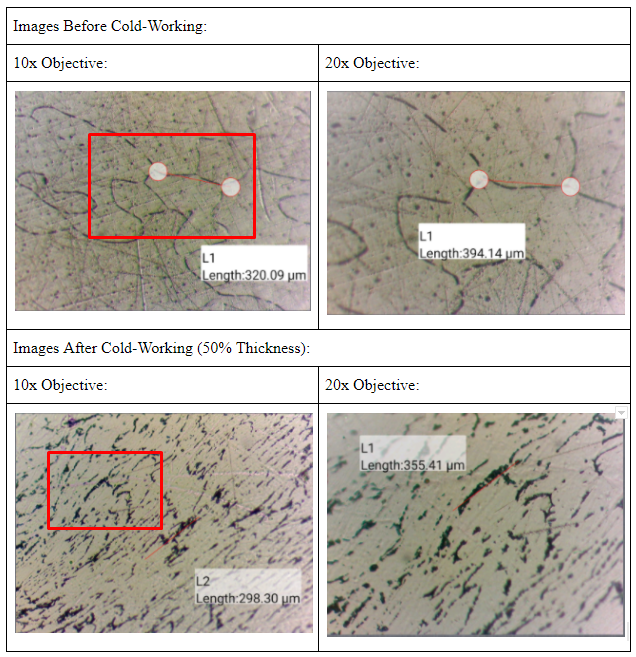
\includegraphics[width=400pt]{ColdWorking.png}
\end{center}

\indent It is apparent that after cold-working, the images in the microscope show a different type of composition of granular patterns. When the original sample was viewed, each of the grains connected and created irregular but closed shapes within the aluminum. After cold-working the metal, the grains overlap and spread across the whole surface. There are more visual grain marks, but less form to their presence. Using the scales, the grains appear to have broken apart into more smaller sections in the cold-worked samples. The grains are also all positioned to flow in the same direction, which may have been the reason the hardness increased. 

\indent Our hypothesis was disproved after doing the experiment. Annealing a metal actually lowered its hardness, and cold-working a metal into a thinner thickness increased the hardness. This can be best displayed using the objective lens images taken where the grains are far less structured after cold working. Annealing undoes the process of cold-working.


\section{Broader Impacts}

\begin{enumerate}
\item Look up the differences in terms of composition and physical properties for both the 3003 and 6061 alloys, make a table. In your research you should find that the 6061 alloy is heat treatable aluminum alloy will the 3003 is non-heat treatable. What is the significance of this designation? Does this explain the differences observed in these alloys during the your cold working and heat treating experiment?   

\begin{center}
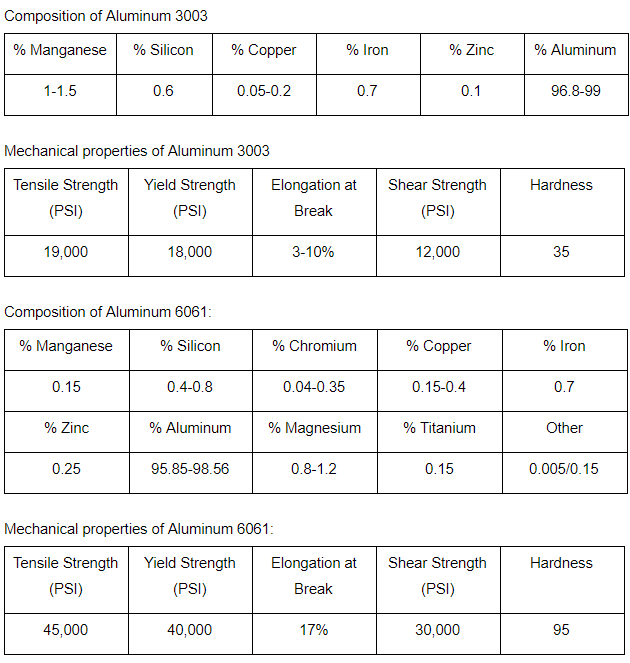
\includegraphics[width=400pt]{BroaderImpact1.png}
\end{center}

\paragraph{}
The annealing process done during the experiment decreases the hardness of Aluminum 6061. Annealing can also be used to soften the material, thus improve the properties of cold working. After an hour of heating, the hardness of the sample was reduced providing further evidence of this application. This means that the material will elongate much further during cold rolling due to the increased ductility.

\item How might you expect the observed changes in mechanical properties following cold work to affect the properties and performance of aluminum automotive body panel? Consider that aluminum panels undergo significant cold work during the stamping process used to form initially flat sheets of aluminum into a heavily curved body panels such as a fender. How might temperature be used to modify the properties of the final part following forming? 

\paragraph{}
Cold rolling the aluminum body panels of an automobile would increase the strength of the
material, as well as decreasing the ductility.  The decreased ductility may prove to be slightly more hazardous, as the material will not be able to crumple and thus absorb the energy applied to the car during an accident. However, the increased strength of the panel after cold rolling my be enough to offset this potential danger. Baking the panel after it was first cold rolled could potentially reduce the brittleness of the part, and would make it a more usable piece than if it was just a sheet of stiff, rigid aluminum.  Temperature will also make the material tougher than it was before. In the event of a crash, this will allow the panel to absorb more energy and deform plastically with a decreased chance of the panel fracturing.



\end{enumerate}


\end{document}